\chapter{Keycloak}

\section{Introduction}
Keycloak is a very popular open-source single sign-on and identity and access management solution for modern applications and services.
The goal of Keycloak is to simplify security so that it is easy for application developers to secure the apps and services they have deployed in their organization.
Security features that developers normally have to write for themselves are provided out of the box and are easily tailorable to the individual requirements of your organization.

Keycloak provides customizable user interfaces for login, registration, administration, and account management.
You can also use Keycloak as an integration platform to hook it into existing LDAP and Active Directory servers.
You can also delegate authentication to third-party identity providers like Facebook and Google.

This community project is currently, in 2024, under the stewardship of the Cloud Native Computing Foundation (CNCF).\cite{keycloak-web}

\newpage
\section{Service Provider Interface}\label{keycloak-spi}
Service Provider Interface (SPI) is an API intended to be implemented or extended by a third party.
It can be used to enable framework extension and replaceable components.\cite{keycloak-spi}

SPI is an essential tool for developers to customize different aspects of Keycloak as per their specific requirements.
Using SPI, developers can create their own Keycloak extensions and modify functionalities such as the login screen appearance, adding new authentication methods, or integrating with different credential stores.

SPI allows developers to adapt Keycloak to diverse environments and business needs.
This includes enhancing security measures, integrating with different databases, or improving the overall user experience. Essentially, SPI empowers developers to extend Keycloak beyond its original functionalities, making it adaptable and versatile across a range of scenarios.

\subsection{Necessary Parts}
In order to properly implement custom SPI for Keycloak, it is necessary to comply with the approach Keycloak suggests.
The essential parts of the custom SPI are new classes that implement these interfaces:
\begin{itemize}
    \item \textit{Spi}
    \item \textit{Provider}
    \item \textit{ProviderFactory}
\end{itemize}

A specific implementation of the \textit{Spi} interface provides some sort of wrapper for the whole custom SPI representation with the required specification of provider class and provider factory class.
Besides that, certain other attributes are present, such as name and flag, used to determine whether the SPI is internal or not.

A specific implementation of the \textit{ProviderFactory} interface provides the functionality to create instances of the \textit{Provider} classes.
The \textit{ProviderFactory} follows the Factory design pattern, and only one factory exists for the server.
It supplies a shared configuration used for the creation of new providers, as it does not have to be evaluated or obtained for every single creation of the particular providers.

Additionally, users are able to change only the behavior for the creation of providers by implementing different provider factories, which brings more freedom to the development.

A specific implementation of the \textit{Provider} interface provides an actual object with the capability of bringing a particular business value to the application.
The new provider object is created for every request made to Keycloak, as its lifespan is limited by the request execution.

Keycloak uses the concept of leveraging \textit{Service Loader} for discovering all implementations of the \textit{Spi}, \textit{Provider}, and \textit{ProviderFactory} interfaces.
Basically, in order to use the custom providers and factories, they need to be registered in the application.
It is done through the specification of class names of the providers and factories in files located in the `META-INF/services` folder.

\subsection{Configuration}
Keycloak nourishes the ability to configure all available SPIs through the dynamically assembled configuration properties.
In that case, changing the particular value of a specific provider implementation is achievable.
Enabling and disabling particular providers is also possible.\cite{keycloak-spi-config}
\newline
\newline
Providers can be configured by using a specific configuration format such as follows:

\begin{align}
    $spi-<spi-id>-<provider-id>-<property>=<value>$
\end{align}
\newline
\newline
Where the explanation of these items is as follows:
\begin{itemize}
    \item \textit{<spi-id>} is the name of the SPI you want to configure.
    \item \textit{<provider-id>} is the id of the provider you want to configure.
    \item \textit{<property>} is the actual name of the property you want to set for a given provider.
\end{itemize}

\section{Authentication Flow}
Authentication flow is a container for all authentications, screens, and actions that must happen during login, registration, and other Keycloak workflows.
It is essentially a step-by-step process that users need to go through during authentication.

For instance, a login flow outlines the necessary credentials a user needs to provide to gain access.
Similarly, a registration flow dictates the required profile information a user must provide, and whether additional measures like reCAPTCHA are necessary to prevent bot activity.

Additionally, a credential reset flow specifies the actions a user must take before being able to reset their password. \cite{keycloak-auth-flows}

\newpage
\section{Authentication Execution}
Authentication executions are the foundational elements of Authentication flows.
They empower administrators to craft tailored authentication processes for specific needs.
These executions allow for the creation of comprehensive authentication flows, providing flexibility and control to address various scenarios effectively.

By orchestrating a series of steps and actions, administrators can ensure secure authentication while accommodating diverse user requirements.
The modular nature of authentication executions enables administrators to mix and match components, facilitating adaptability and reusability.
Ultimately, authentication executions serve as the cornerstone for building robust and user-centric authentication experiences within systems.

Authentication executions may play different roles in the context of particular authentication flows and provide the ability to control authentication flows in a more fine-grained way. \cite{keycloak-auth-flows}
\newline
\newline
Every authentication execution has a specified requirement type in its parent flow as follows:

\begin{enumerate}
    \item \textbf{Required} -- all \textit{required} elements in the flow must be successfully sequentially executed. The flow terminates if a \textit{required} element fails.
    \item \textbf{Alternative} -- a single element needs to execute successfully for the flow to be considered successful. If a flow includes \textit{required} elements, they alone determine its success, rendering any \textit{alternative} elements within it unnecessary.
    \item \textbf{Disabled} -- the element does not count to mark a flow as successful.
    \item \textbf{Conditional} -- (only set on sub-flows) if all executions evaluate as \textit{true}, the \textit{conditional} sub-flow acts as \textit{required}, otherwise \textit{disabled}.
\end{enumerate}

\newpage

\section{Basic Authentication Flow}
Authentication flows in Keycloak are very flexible and can address the unique needs of organizations.
To illustrate the relationships between flows, sub-flows, and executions, Keycloak renders a graph with these elements, as shown in the picture below.

The authentication flow contains several authentication flows and authentication executions.
In the graph, every sub-flow is noted by a circle with the inner text \textit{Start <auth-flow-name>}, and the end of the sub-flow by a circle with the inner text \textit{End <auth-flow-name>}.

The flow contains on the first level 3 elements as \textit{Cookie}, \textit{Kerberos}, and flow \textit{WebAuthn forms}.
These elements are marked as alternatives, and if one of them succeeds, the authentication can proceed.
When the \textit{Cookie} and \textit{Kerberos} executions are not fulfilled, the \textit{WebAuthn forms} flow starts.

When a user provides their credentials via the Passwordless WebAuthn authenticator, the authentication is successful.
Otherwise, a user needs to provide their password and then biometrics via the WebAuthn authenticator.

\begin{figure}[htbp]
  \centering
  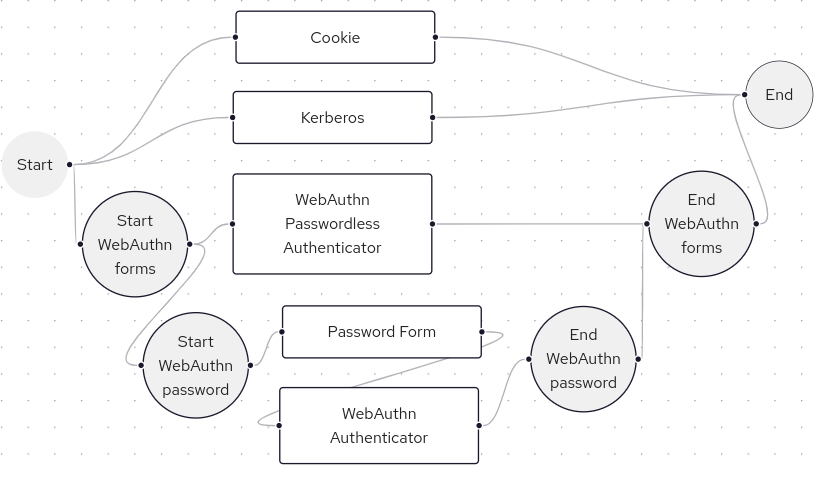
\includegraphics[width=1\textwidth]{img/flow-new.png}
  \caption{WebAuthn Flow}
  \label{fig:basic-auth-flow}
\end{figure}

\Blindtext